\section[\englishfont 4 研究成果总结]{研究成果总结}

\begin{frame}{论文发表}
\newBackground
\frametitle{论文发表 (第一作者或二作 (导师一作)\hspace{0.5em}\textcolor{red}{7}\hspace{0.5em}篇,另有\hspace{0.5em}\textcolor{red}{2}\hspace{0.5em}篇在投)}
\begin{center}
\begin{textblock*}{\textwidth}(-1.1cm,1.85cm)
\begin{minipage}[t]{0.83\textwidth}
\begin{itemize}
\setlength{\itemsep}{1pt}
\setlength{\parskip}{0pt}
\setlength{\parsep}{0pt}
	\begin{small}
	\item[1] \englishfont \underline{\textcolor{cqublue}{XU X}}, LIU K, DAI P, et al. Joint task offloading and resource optimization in NOMA-based vehicular edge computing: A game-theoretic DRL approach[J]. \textcolor{cqublue}{Journal of Systems Architecture} (\textcolor{red}{JSA}), 2023. (中科院SCI 2区)
	\item[2] \underline{\textcolor{cqublue}{许新操}}, 刘凯, 刘春晖, 等. 基于势博弈的车载边缘计算信道分配方法[J]. \textcolor{red}{电子学报}, 2021. (CCF T1类中文期刊)
	\item[3] \underline{\textcolor{cqublue}{XU X}}, LIU K, XIAO K, et al. Vehicular fog computing enabled real-time collision warning via trajectory calibration[J]. \textcolor{cqublue}{Mobile Networks and Applications} (\textcolor{red}{MONET}), 2020. (中科院SCI 3区)
	\item[4] LIU K, \underline{\textcolor{cqublue}{XU X}}, CHEN M, et al. A hierarchical architecture for the future Internet of Vehicles[J]. \textcolor{cqublue}{IEEE Communications Magazine} (\textcolor{red}{ComMag}), 2019. (中科院SCI 1区)
	\item[5] \underline{\textcolor{cqublue}{XU X}}, LIU K, ZHANG Q, et al. Age of view: A new metric for evaluating heterogeneous information fusion in vehicular cyber-physical systems[C]. \textcolor{red}{IEEE ITSC}, 2022. (智能交通领域重要会议)
	\item % 解决最后一个item行间距问题
	\end{small}
\end{itemize}
\end{minipage}
\end{textblock*}
\end{center}
\begin{center}
\begin{textblock*}{\textwidth}(7cm,1.85cm)
\begin{minipage}[t]{0.4\textwidth}
\begin{figure}
  \centering
  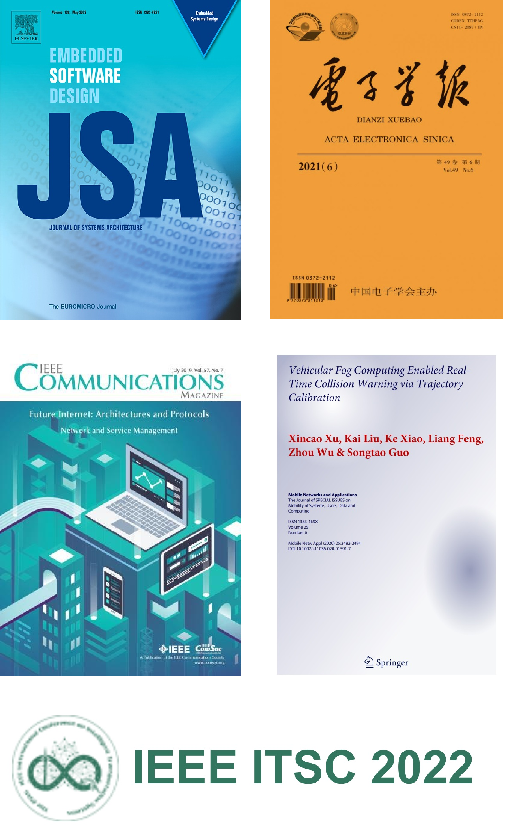
\includegraphics[width=0.65\textwidth]{fig/publication1.pdf}
\end{figure}
\end{minipage}
\end{textblock*}
\end{center}
\end{frame}

\begin{frame}{论文发表}
\newBackground
\frametitle{论文发表 (第一作者或二作 (导师一作)\hspace{0.5em}\textcolor{red}{7}\hspace{0.5em}篇,另有\hspace{0.5em}\textcolor{red}{2}\hspace{0.5em}篇在投)}
\begin{center}
\begin{textblock*}{\textwidth}(-2cm,1.85cm)
\begin{minipage}[t]{0.7\textwidth}
	\begin{itemize}
	\begin{small}
	\item[6] \englishfont \underline{\textcolor{cqublue}{许新操}}, 周易, 刘凯, 等. 车载雾计算环境中基于势博弈的分布式信道分配[C]. \textcolor{cqublue}{CWSN}, 2020. (最佳论文候选)
	\item[7] \underline{\textcolor{cqublue}{XU X}}, LIU K, XIAO K, et al. Design and implementation of a fog computing based collision warning system in VANETs[C]. \textcolor{cqublue}{IEEE ISPCE-CN}, 2018. (最佳论文奖)
	\item[8] \underline{\textcolor{cqublue}{XU X}}, LIU K, DAI P, et al. Cooperative sensing and heterogeneous information fusion in VCPS: A multi-agent deep reinforcement learning approach[J]. \textcolor{cqublue}{IEEE Transactions on Intelligent Transportation Systems} (\textcolor{red}{T-ITS}), under major revision. (中科院SCI 1区)
	\item[9] LIU K,\underline{\textcolor{cqublue}{XU X}}, DAI P, et al. Cooperative sensing and uploading for quality-cost tradeoff of digital twins in VEC[J]. \textcolor{cqublue}{IEEE Transactions on Consumer Electronics} (\textcolor{red}{TCE}), under minor revision. (中科院SCI 2区)
	\item % 解决最后一个item行间距问题
	\end{small}
\end{itemize}
\end{minipage}
\end{textblock*}
\end{center}

\begin{center}
\begin{textblock*}{\textwidth}(5.9cm,1.85cm)
\begin{minipage}[t]{0.4\textwidth}
\begin{figure}
  \centering
  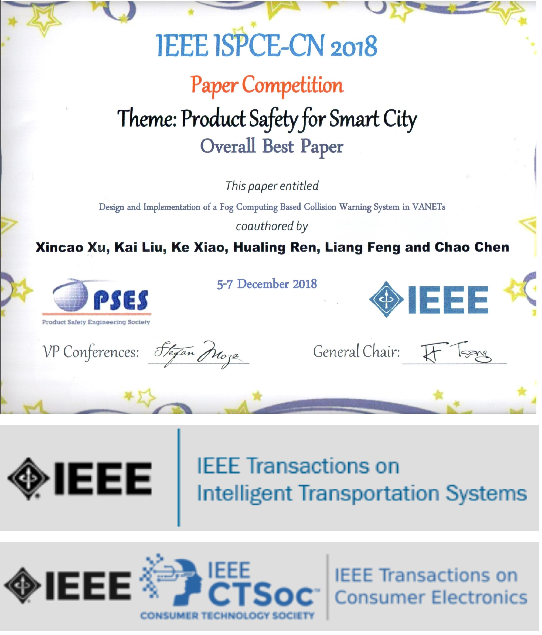
\includegraphics[width=0.9\textwidth]{fig/publication2.pdf}
\end{figure}
\end{minipage}
\end{textblock*}
\end{center}

\end{frame}

\begin{frame}{论文发表}
\newBackground
\frametitle{论文发表 (合作作者\hspace{0.5em}\textcolor{red}{6}\hspace{0.5em}篇)}
\begin{center}
\begin{textblock*}{\textwidth}(1cm,1.85cm)
	\begin{footnotesize}
		\begin{itemize}
			\item[1] \englishfont LIU C, LIU K, REN H, \underline{\textcolor{cqublue}{XU X}}, et al. RtDS: Real-time distributed strategy for multi-period task offloading in vehicular edge computing environment[J]. \textcolor{cqublue}{Neural Computing and Applications}, to appear. (中科院SCI 2区)
			\item[2] XIAO K, LIU K, \underline{\textcolor{cqublue}{XU X}}, et al. Cooperative coding and caching scheduling via binary particle swarm optimization in software defined vehicular networks[J]. \textcolor{cqublue}{Neural Computing and Applications}, 2021. (中科院SCI 2区)
			\item[3] XIAO K, LIU K, \underline{\textcolor{cqublue}{XU X}}, et al. Efficient fog-assisted heterogeneous data services in software defined VANETs[J]. \textcolor{cqublue}{Journal of Ambient Intelligence and Humanized Computing}, 2021. (中科院SCI 3区)
			\item[4] LIU C, LIU K, \underline{\textcolor{cqublue}{XU X}}, et al. Real-time task offloading for data and computation intensive services in vehicular fog computing environments[C]. \textcolor{cqublue}{IEEE MSN}, 2020. (CCF C类国际会议)
			\item[5] ZHOU Y, LIU K, \underline{\textcolor{cqublue}{XU X}}, et al. Multi-period distributed delay-sensitive tasks offloading in a two-layer vehicular fog computing architecture[C]. \textcolor{cqublue}{NCAA}, 2020. (EI 索引)
			\item[6] ZHOU Y, LIU K, \underline{\textcolor{cqublue}{XU X}}, et al. Distributed scheduling for time-critical tasks in a two-layer vehicular fog computing architecture[C]. \textcolor{cqublue}{IEEE CCNC}, 2020. (EI 索引)
			\item % 解决最后一个item行间距问题
		\end{itemize}	
	\end{footnotesize}
\end{textblock*}
\end{center}
\end{frame}

\begin{frame}{代码开源}
\newBackground
\frametitle{\englishfont 代码开源 (获得 100+ GitHub Stars)}
\begin{minipage}[t]{0.6\textwidth}
	\begin{itemize}
		\begin{footnotesize}
			\item[1] 基于差分奖励的多智能体强化学习源代码\\ \href{https://github.com/neardws/Multi-Agent-Deep-Reinforcement-Learning}{\tiny \englishfont https://github.com/neardws/Multi-Agent-Deep-Reinforcement-Learning}
			\item[2] 基于博弈理论的多智能体强化学习源代码\\ \href{https://github.com/neardws/Game-Theoretic-Deep-Reinforcement-Learning}{\tiny \englishfont https://github.com/neardws/Game-Theoretic-Deep-Reinforcement-Learning}
			\item[3] 基于多目标的多智能体强化学习源代码\\ \href{https://github.com/neardws/MAMO-Deep-Reinforcement-Learning}{\tiny \englishfont https://github.com/neardws/MAMO-Deep-Reinforcement-Learning}
			\item[4] 基于视图校准的碰撞预警源代码\\ \href{https://github.com/neardws/fog-computing-based-collision-warning-system}{\tiny \englishfont https://github.com/neardws/fog-computing-based-collision-warning-system}
			\item[5] 基于C-V2X通信的碰撞预警原型系统实现源代码\\ \href{https://github.com/neardws/V2X-based-Collision-Warning}{\tiny \englishfont https://github.com/neardws/V2X-based-Collision-Warning}
			\item[6] 滴滴GAIA数据集处理源代码\\ \href{https://github.com/neardws/Vehicular-Trajectories-Processing-for-Didi-Open-Data}{\tiny \englishfont https://github.com/neardws/Vehicular-Trajectories-Processing-for-Didi-Open-Data}
			\item % 解决最后一个item行间距问题
		\end{footnotesize}
	\end{itemize}
\end{minipage}%
\begin{minipage}[t]{0.3\textwidth}
\begin{figure}
  \centering
  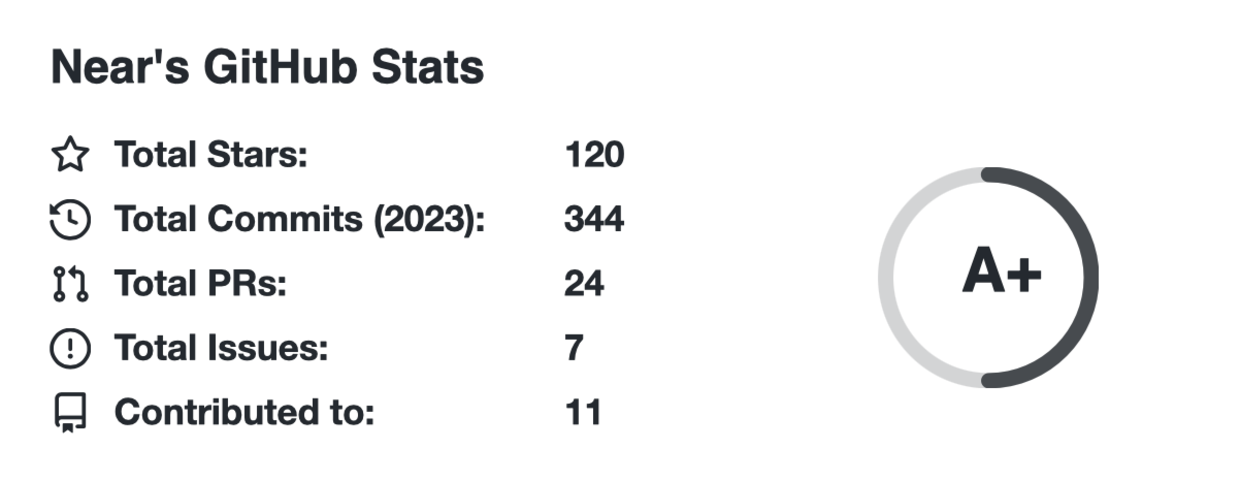
\includegraphics[width=1.2\textwidth]{fig/github_stars.pdf}
\end{figure}
\begin{figure}
  \centering
  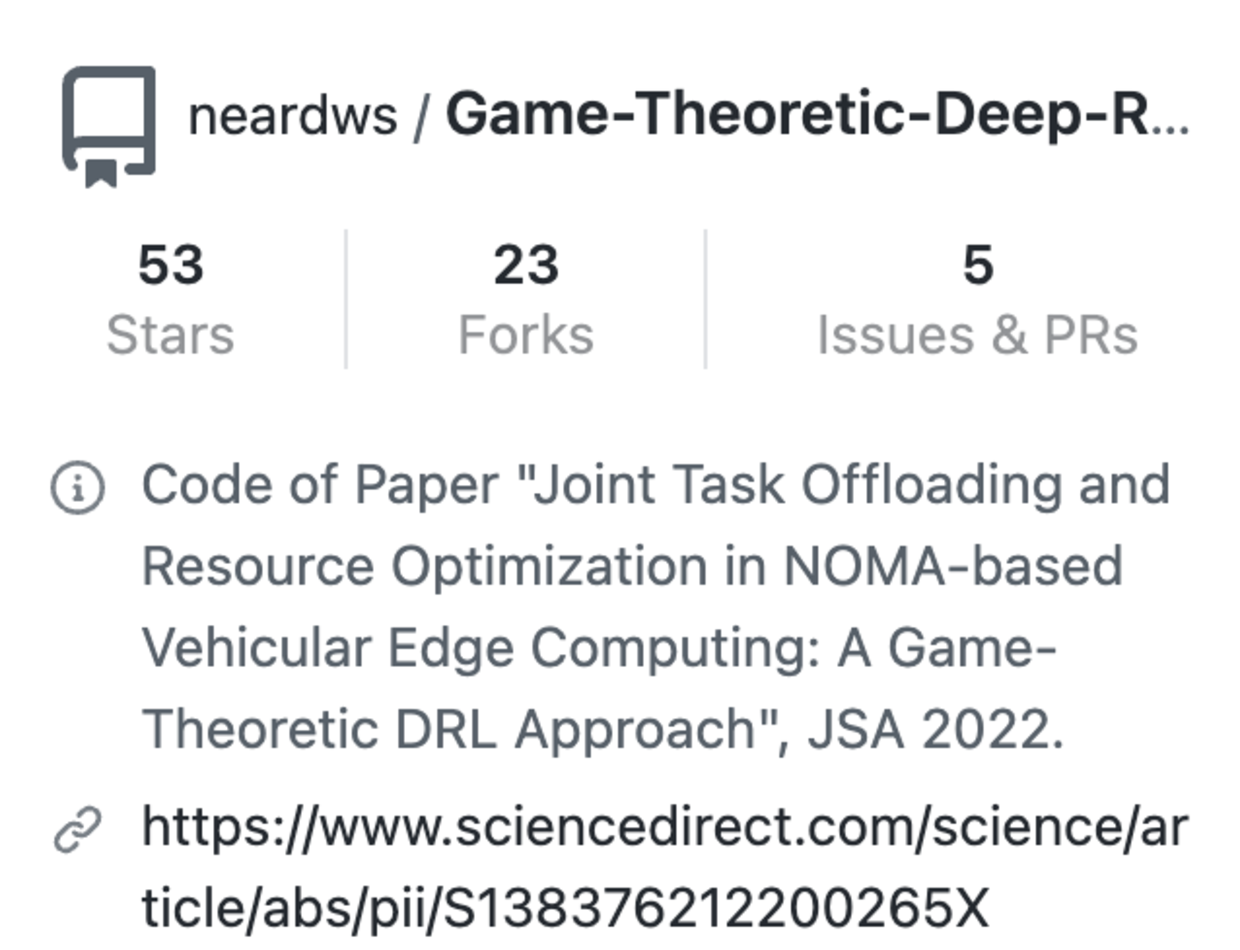
\includegraphics[width=1\textwidth]{fig/github_gtdrl.pdf}
\end{figure}
\end{minipage}	
\end{frame}

\begin{frame}{科研项目与专利}
\newBackground
\begin{center}
\begin{textblock*}{\textwidth}(1cm,1.85cm)
\begin{itemize} \englishfont
	\item[\ding{111}] 参与科研项目
		\begin{itemize} 
		\begin{footnotesize}
			\item[\ding{226}] \textcolor{cqublue}{国家自然科学基金面上项目},“面向车联网边缘智能的计算模型部署与协同跨域优化”,项目编号: 62172064,2022/01–2025/12. (在研)
			\item[\ding{226}] \textcolor{cqublue}{国家自然科学基金面上项目},“面向大规模数据服务的异构融合车联网架构与协议研究”,项目编号: 61872049,2019/01–2022/12. (结题)
		\end{footnotesize}
		\end{itemize}
	\item[\ding{111}] 申请发明专利
		\begin{itemize}
		\begin{footnotesize}
			\item[\ding{226}] \underline{\textcolor{cqublue}{许新操}}, 刘凯, 李东. 一种针对软件定义车联网的控制平面视图构建方法. \textcolor{red}{已授权}. 专利号:ZL202110591822.1.
			\item[\ding{226}] 刘凯, 张浪, \underline{\textcolor{cqublue}{许新操}}, 任华玲, 周易. 一种基于边缘计算的盲区车辆碰撞预警方法. \textcolor{red}{已授权}. 专利号:ZL201910418745.2.
			\item[\ding{226}] 任华玲, 刘凯, 陈梦良, 周易, \underline{\textcolor{cqublue}{许新操}}. 一种基于雾计算的信息采集、计算、传输架构. \textcolor{red}{已授权}. 专利号:ZL201910146357.3.
		\end{footnotesize}
		\end{itemize}
	
\end{itemize}
\end{textblock*}
\end{center}
\end{frame}

\begin{frame}{盲审意见与修改情况}
\newBackground
\begin{center}
\begin{textblock*}{\textwidth}(1cm,1.85cm)
\begin{itemize}[itemsep=0.2\baselineskip] \englishfont
	\item[\ding{111}] \textcolor{cqublue}{总体评价 \textbf{A B B}}
	\item[\ding{111}] \textcolor{cqublue}{评审专家 1}
		\begin{itemize}[itemsep=0.2\baselineskip] 
		\begin{small}
			\item[\ding{52}] 车联网分层架构详细阐述
			\item[\ding{52}] VCPS质量定义增加实例
		\end{small}
		\end{itemize}
	\item[\ding{111}] \textcolor{cqublue}{评审专家 2}
		\begin{itemize}[itemsep=0.2\baselineskip] 
		\begin{small}
			\item[\ding{52}] 数据平面和控制平面概念介绍
			\item[\ding{52}] 论文符号定义优化
		\end{small}
		\end{itemize}
		\item[\ding{111}] \textcolor{cqublue}{评审专家 3}
		\begin{itemize}[itemsep=0.2\baselineskip] 
		\begin{small}
			\item[\ding{52}] 排版问题
			\item[\ding{52}] 碰撞预警系统图详细阐述
		\end{small}
		\end{itemize}
\end{itemize}
\end{textblock*}
\end{center}
\end{frame}

\begin{frame}
\newBackground
\Background
    \begin{center} \doublespacing
        {\Huge 致谢}\\
       	\textit{感谢刘凯教授多年的辛勤指导!}\\
       	\textit{感谢各位专家的指导!}\\
       	\textit{感谢所有给予我帮助的老师和同学!}
    \end{center}
\end{frame}

\begin{frame}
\newBackground
\Background
    \begin{center} \doublespacing
        {\Huge 敬请批评指正!}
    \end{center}
\end{frame}